\chapter{Simultaneous Localization And Mapping}
\section{Pose Estimation}
In this chapter, we focus on the use of an embedded visual sensor for pose estimation. These sensors\footnote{The used visual sensors are supposed to be calibrated.}, mounted on-board moving robots, are used to gather information to map the environment and to estimate the robot’s trajectory. To this end, VO and SLAM methods are dominant.
\subsection{Visual Odometry}
\subsubsection{Overview}
The visual odometry process consists in incrementally estimating the pose of a vehicle by examining the changes that motion induces on the images taken from its on-board rigidly attached camera [Scaramuzza and Fraundorfer, 2011]. VO is a 3D motion estimation (translation + rotation) computed from sequential optical sensors data such as images (See Figure 2.1).
\begin{figure}
    \centering
    \begin{subfigure}[h]{0.9\linewidth}
        \centering
        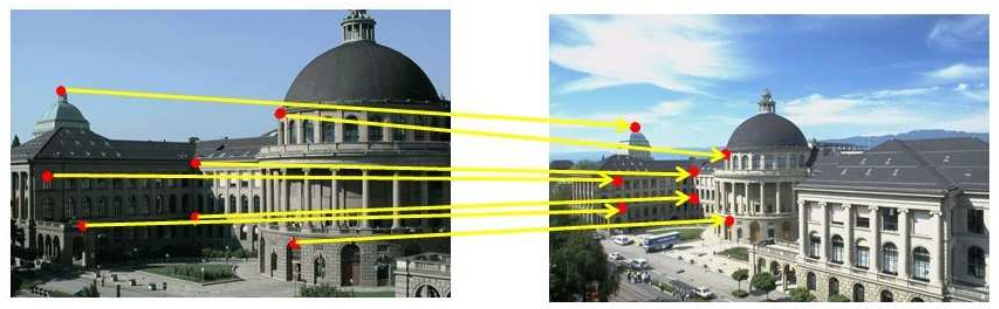
\includegraphics[width=\linewidth]{assets/2_1_a.png}
        \caption{{Consecutive images correspondences.}}
        \label{fig:subfigure1}
    \end{subfigure}
    \hfill
    \begin{subfigure}[h]{0.8\linewidth}
        \centering
        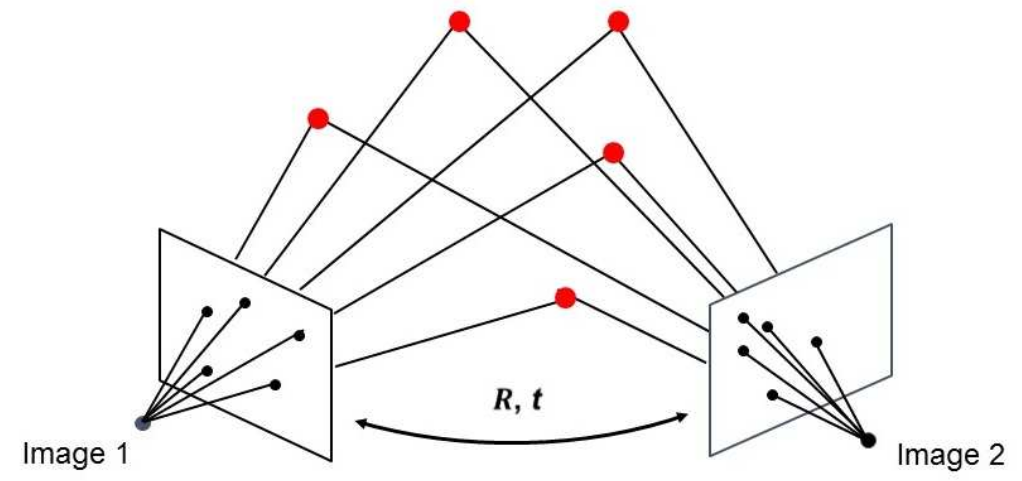
\includegraphics[width=\linewidth]{assets/2_1_b.png}
        \caption{{Consecutive images motion estimation.}}
        \label{fig:subfigure2}
    \end{subfigure}
    \caption{The VO working principle. Images from [Schöps et al., 2014].}
\end{figure}

Assuming static scenes, two consecutive images at time \textit{k} and \textit{k-1} are related by a rigid body transformation $\mathbf{T_\textit{k}}$ in Eq.\ref{eq:2.1}
\begin{equation} \label{eq:2.1}
    \mathbf{T_\textit{k}} = \begin{bmatrix}
        \mathbf{R_\textit{k,k-1}} & \mathbf{t_\textit{k,k-1}} \\
        \mathbf{O_\text{1x3}}     & 1                         \\
    \end{bmatrix}
\end{equation}

Where $\mathbf{T_\mathit{k}} \in \mathbb{R_\text{4x4}}$ in the relative transformation, $\mathbf{R_\mathit{k,k-1}}\in\mathbb{R_\text{3x3}}$ is the rotation made on each axis from the previous pose to the next one, and $\mathbf{t_\mathit{k,k-1}}\in\mathbb{R_\text{3x1}}$ is the translation on the three axes. Figure \ref{fig:2.2} shows an illustration of VO problem formulation where the following sets an be introduced:

\begin{itemize}
    \item $\mathcal{T_\textit{0:n}}=\{\mathbf{T_1},\mathbf{T_2},...,\mathbf{T_\textit{n}}\}$: The set of camera motions.
    \item $\mathcal{C_\textit{0:n}}=\{\mathbf{C_0},\mathbf{C_1},...,\mathbf{C_\textit{n}}\}$: The set of camera poses w.r.t the initial coordinate frame.
\end{itemize}
\begin{figure}[h]
    \centering
    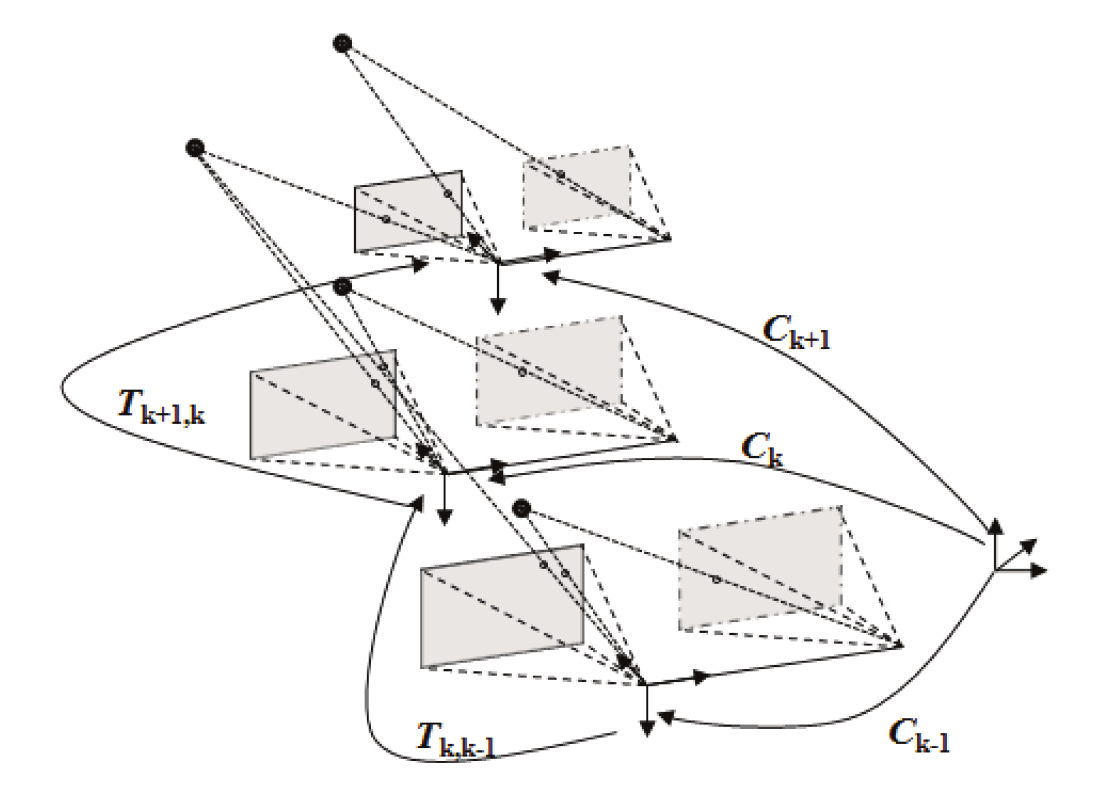
\includegraphics[width=\linewidth]{assets/2_2.png}
    \caption{Illustration of the visual odometry problem. Case of a stereo camera (At time \textit{k}, two boxes representing two image frames are available). Image from Scaramuzza and Fraundorfer, 2011.}
    \label{fig:2.2}
\end{figure}
The VO consists in estimating the transformation $\mathcal{T_\textit{0:n}}$. Then, to recover the camera trajectory $\mathcal{C_\textit{0:n}}$. the computed $\mathcal{T_\textit{0:n}}$ is concatenated using Eq.\ref{eq:2.2} where, the initial camera pose $\mathbf{C_0}$ is arbitrary set.
\begin{equation} \label{eq:2.2}
    \mathbf{C_\textit{n}}=\mathbf{C_\textit{n-1}}\mathbf{T_\textit{n}}
\end{equation}
VO estimation requires assumptions such as:
\begin{itemize}
    \item The environment has to be sufficiently illuminated and structured.
    \item The scene has to be mostly static.
    \item The consecutive frames need sufficient overlap among them.
\end{itemize}
\subsubsection{Related work}
VO can be computed by two approaches classified into: Sparse visual odometry Engel et al., 2016  (where only a part of the image data is used) and dense visual odometry Kerl et al., 2013b (where all the available image data are used). According to Schops et al., 2014, the existing VO methods (also SLAM methods) can be classified into Feature-based method and Direct method (See Figure \ref{fig:2.3}).
\begin{figure}[h]
    \centering
    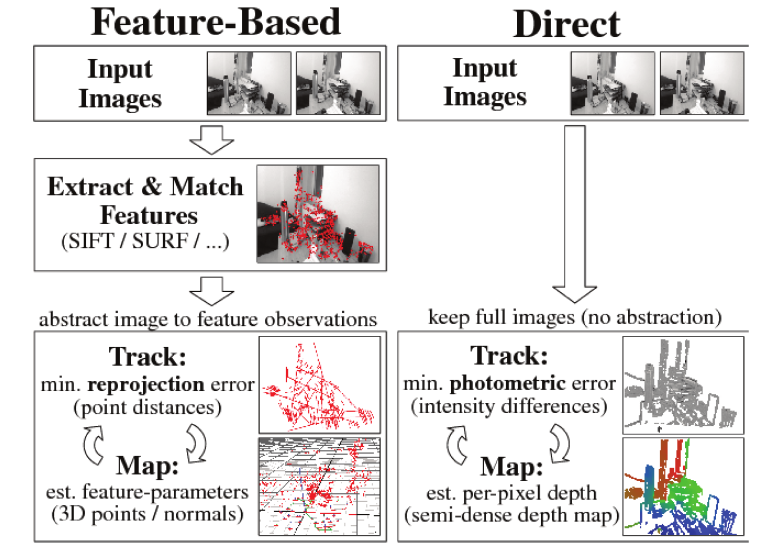
\includegraphics[width=\linewidth]{assets/2_3.png}
    \caption{Feature-based versus direct methods. Image from [Schops et al., 2014]}
    \label{fig:2.3}
\end{figure}\\
The feature-based methods abstract images to features and discard all the order information. The main pipeline of these methods are:
\begin{itemize}
    \item To acquire the image sequences.
    \item To detect/extract the features using approaches such as Scale-Invariant Feature Transform (SIFT) or Speed Up Robust Features (SURF).
    \item To match/track the features using techniques such as RANdom SAmple Consensus (RANSAC)
    \item To estimate the relative motion between the features (2D/2D, 3D/3D, 3D/2D)
    \item To optimize the estimated transformation.
\end{itemize}
These steps may slightly differ depending on the adopted method. For example, the bundle adjustment-based approach is a commonly used feature-based method where the main steps [Sibley et al., 2010, Shade and Newman, 2011] are:
\begin{itemize}
    \item Image processing: To remove the distortion in lens and to filter the images to allow faster matching of features.
    \item Image alignment: To make an initial estimate of a 3D rotation using a gradient descent method-based on image intensity.
    \item Feature match in time: To project the 3D features into the left and the right images and match them using a sum-absolute-difference error metric.
    \item Initialize new features: To track about 100 to 150 features and to ensure a spatial distribution using a quad-tree.
\end{itemize}
Results, presented in [Shade and Newman, 2011], have shown that these estimations are robust even under difficult conditions. They are mostly adapted for large scale environments.\\ \\
The direct methods [Schöps et al., 2014] perform tracking directly on the image intensity
(instead of extracting and matching features). This allows to achieve a higher accuracy
and robustness, especially in indoor environments where only few features are available.
But, this method requires a powerful Graphic Processing Unit (GPU) to run in real time.\\\\
According to [Fang and Scherer, 2014, Fang and Zhang, 2015], the VO for RGB-D sensor
can be classified within three categories:
\begin{itemize}
    \item The image-based category [Huang et al., 2011, Kerl et al., 2013b, Endres et al., 2014, Li et al., 2015] that uses RGB-D and depth data. It is mostly adapted when there is a good gray image value or visual features.
    \item The depth-based category [Wang et al., 2017] that uses point cloud and is commonly used in featureless or dark environment.
    \item The hybrid category [Zhang et al., 2014] that uses point cloud and RGB-D.
\end{itemize}
The Fovis presented in [Huang et al., 2011], is a feature-based VO method that provides consistent motion estimation but needs to work at high frequencies for a correct estimation.\\\\
The Dense VO method (DVO), introduced in [Steinbrücker et al., 2011], estimates dense
VO directly from the RGB-D frame by minimizing the difference between the previous
image and the back-projected current RGB-D image. This approach is optimized in [Kerl
        et al., 2013b] by a probabilistic derivation and the possibility of prior integration of the
motion and the sensor noise. It has been extended by adding weight to each pixel and by incorporating a motion prior. Actually, this method is based on the photo-consistency
assumption that assumes that if a point is observed by two cameras, it has the same
brightness in both images.\\\\
Authors in [Zhang et al., 2014] propose the Depth Enhanced Monocular Odometry method
(DEMO) to enhance VO from monocular images by the assistance of depth information
even if it is sparsely or locally unavailable. According to [Fang and Scherer, 2014, Zhang
        et al., 2014, Fang and Zhang, 2015], DVO is adapted for environment with relatively dark
illumination and DEMO [Zhang et al., 2014] for areas with no sufficient depth information.\\\\
A Fast Semi-Direct Monocular Visual Odometry called SVO is proposed in [Forster et al.,
        2014]. The algorithm operates directly on pixel intensities. The 3D points are estimated
using probabilistic mapping method that allows to reduce the outliers (false matching
points) and get more reliable points. Results show that the proposed method is robust,
and faster than current state-of-the-art methods.\\\\
In some works, authors use Structure From Motion (SFM) term as a synonym of VO.
Actually, VO is a particular case of SFM [Scaramuzza and Fraundorfer, 2011]. In fact,
SFM is a more general process that treats both 3D problem of camera pose estimation and
structure from images set that can even be unordered. They are generally refined with an
off-line optimization known as bundle adjustment. The SFM’s computation time grows
when the image number grows too. Compared to the SFM, VO focuses on 3D sequential
pose estimation in real time. In VO, the trajectory estimation optimization is optional.
\subsection{Simultaneous Localization And Mapping (SLAM)}
\subsubsection{Overview}
The SLAM problem is one of the most important topics in the robotic community. It
consists in answering simultaneously two important questions: Where is the robot? And
what does the world looks like? Let’s consider a robot with a visual sensor mounted on
it. It is moving in an a priori unknown environment and is collecting information about
relative observations of landmarks. Figure \ref{fig:2.4} shows the evolution of the robot poses
and landmarks during a short time of navigation [Durrant-Whyte and Bailey, 2006]. The
following sets are then introduced:
\begin{itemize}
    \item $\mathcal{P_\textit{0:k}}=\{\mathbf{p_0},\mathbf{p_1},...,\mathbf{p_\textit{k}}\}$ represents the set of poses of robot. Each pose includes the position and the orientation of the robot.
    \item $\mathcal{U_\textit{0:k}}=\{\mathbf{u_1},\mathbf{u_2},...,\mathbf{u_\textit{k}}\}$ represents the set of control vectors used to drive the robot from state $\textit{l}-1$ to state $\textit{l}$ at time $\textit{l}$ with $\textit{l} \in [1..\textit{k}]$
    \item $\mathcal{M_\textit{0:k}}=\{\mathbf{m_1},\mathbf{m_2},...,\mathbf{m_\textit{k}}\}$ represents the set of vectors that defines the states of landmarks. These locations are considered as time invariant.
    \item $\mathcal{Z_\textit{0:k,i}}=\{\mathbf{z_\textit{1,i}},\mathbf{u_\textit{2,i}},...,\mathbf{u_\textit{k,i}}\}$ represents the set of observations of the landmark $\textit{i}$ made at times $[0..\textit{k}]$
\end{itemize}
\begin{figure}[H]
    \centering
    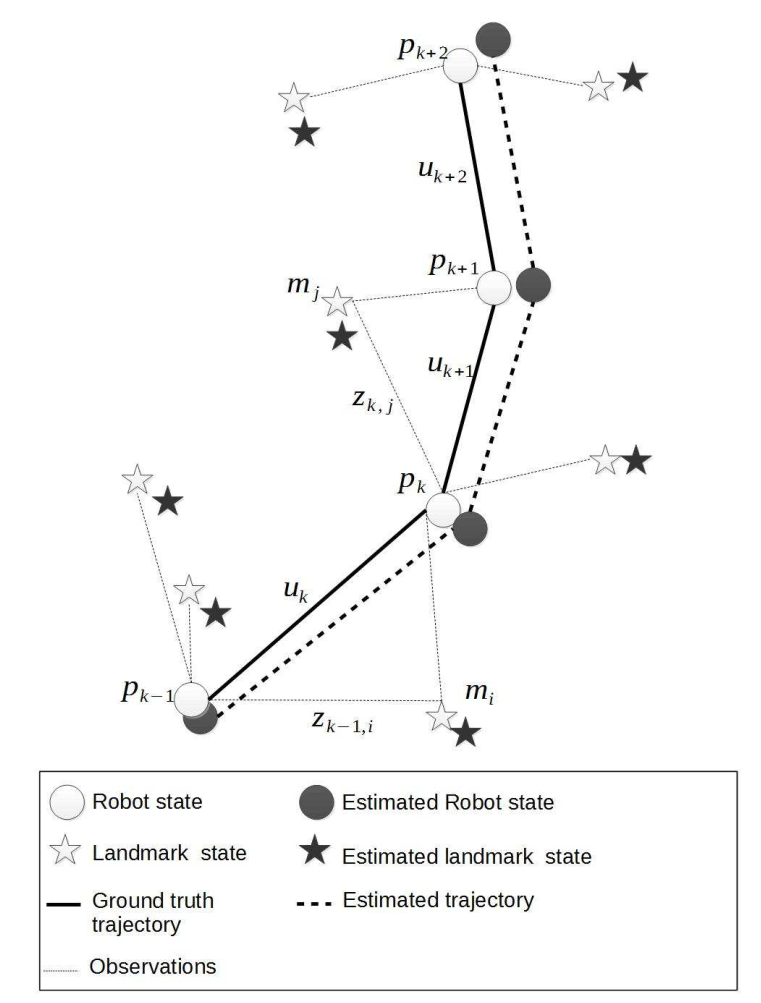
\includegraphics[width=\linewidth]{assets/2_4.png}
    \caption{SLAM problem formulation.}
    \label{fig:2.4}
\end{figure}
The formulation of a probabilistic SLAM can be written in a probabilistic form as expressed in Eq.\ref{eq:2.3}. This probability distribution has to be computed at each time k, knowing the observed landmarks, the control vectors, and the initial robot pose.
\begin{equation} \label{eq:2.3}
    P(\mathbf{p_\mathit{k}},\mathbf{m} \vert \mathcal{Z_\text{0:\textit{k}}},\mathcal{U_\text{0:\textit{k}}},\mathbf{p_0})
\end{equation}
Generally, the SLAM problem is resolved through a recursive solution that requires a motion model and an observation model. By far, the most commonly used approaches for these model representations are:
\begin{itemize}
    \item The Extended Kalman Filter (EKF) for an EKF-SLAM solution.
    \item The Rao-Blackwellised particle filter for a Fast-SLAM solution.
\end{itemize}
Some other solutions, explained in the next section, are proposed to attempt to solve the SLAM problem [Cadena et al., 2016].
\subsubsection{Related work}
The VO’s main objective is to ensure a local consistency while SLAM aims at a global consistency of the map [Renaudeau et al., 2018] and the trajectory [Mur-Artal and Tardós, 2017a]. Indeed, SLAM is used to obtain a global and consistent estimate of the robot path based on loop closure. It allows the algorithm to apply a global optimization to reduce drift on both the trajectory and the map. Whereas, VO aims at estimating the trajectory pose after pose, and applying optimization after a certain number of poses called windowed optimization. The choice between using VO and Visual SLAM is based on a trade-off between performance and consistency, and simplicity of implementation.\\\\
The Parallel Tracking and Mapping (PTAM) proposed in [Klein and Murray, 2007] is a monocular SLAM based on a parallel framework that includes a tracker and a mapper, in order to increase the responsiveness and robustness of the whole system. The tracker enables fast camera localization in real time; whereas keyframe based mapper builds the global map. Authors in [Ta et al., 2013] modified PTAM – originally designed for augmented reality – making it more suitable for robot navigation. Instead of using a motion model, odometry and visual measurements are fused into the framework to deal with the lack of visual features and the lack of motion in the environment. In addition, a loop closer mechanism is performed.\\\\
Authors in [Cunningham et al., 2010] use an extending Smoothing And Mapping (SAM) approach consisting on a graphical model approach that introduces the Constrained Factor Graph (CFG). A Decentralized Data Fusion-SAM (DDF-SAM), that satisfies the DDF requirements while taking into account the benefits of naive approach, is proposed. The framework is composed of three modules:
\begin{itemize}
    \item The Local Optimizer Module performs the SLAM for one robot in its local environment and produces its local map and condensed local graph.
    \item The Communication Module shares the previous condensed local graph so that each robot maintains its local graph and a cache of neighboring robots’ condensed graphs.
    \item The Neighborhood Optimizer Module merges the condensed graphs to obtain a neighborhood graph that can be used to build the map.
\end{itemize}
By applying loop closing process along with DVO method, authors in [Kerl et al., 2013a] propose a SLAM method that applies a global optimization to reduce drift on both the trajectory and the map. Yet, many implementation issues of this SLAM method rise due to versions incompatibility.\\\\
Authors in [Forster et al., 2013a] propose a distributed monocular SLAM for a multi- robot system. To determine each robot’s individual motion, measurements from an on- board camera and Inertial Measurement Unit (IMU) are combined together. Specific data such as image coordinates, descriptors as features of selected keyframes, and relative pose estimation are streamed to a ground station – called Collaborative Structure From Motion (CSFM) – where a map for each robot is created and merged if there is an overlap among them.\\\\
A software architecture is proposed in [Brand et al., 2014] to perform a distributed SLAM. The on-board stereo-vision based mapping system proves its effectiveness in indoor, unstructured outdoor as well as mixed environment.\\\\
A novel direct and feature-less Large-Scale Direct monocular SLAM (LSD-SLAM) method is proposed in [Engel et al., 2014]. It performs an accurate pose estimation using direct image alignment along with filtering-based estimation of semi-dense depth maps. A 3D reconstruction of the environment is represented as a pose graph where keyframes are vertices.\\\\
The OKVIS SLAM [Leutenegger et al., 2015] proposes a non-linear optimization approach that tightly fuses visual measurements along with readings from an IMU. This allows to significant advantages in quality of performance and computational complexity.\\\\
A novel tightly coupled visual-inertial SLAM system is proposed in [Mur-Artal and Tardós, 2017b]. This system is able to be applied to monocular as well as stereo and RGB-D sensors. It performs loop closing to attempt a zero-drift localization in already mapped areas.\\\\
Authors in [Mur-Artal and Tardós, 2017a] propose a lightweight RGB-D feature-based SLAM method called ORB-SLAM2. It is adapted for monocular (depth triangulated from different view), stereo and RGB-D sensors. Using the TUM RGB-D data-set [Sturm et al., 2012], in most cases, ORB-SLAM2 performs better than Elastic-Fusion [Whelan et al., 2016], kintinuous [Whelan et al., 2015], DVO SLAM [Kerl et al., 2013a] and RGB- D SLAM [Endres et al., 2014] in terms of Root Mean Square Error (RMSE) translation error.\\\\
A new open framework for research in Visual Inertial (VI) mapping and localization – called Maplab – is proposed in [Schneider et al., 2018]. It contains a RObust Visual Inertial Odometry (ROVIO) with Localization Integration (ROVIOLI) and an off-line Maplab-console. ROVIOLI, composed of an on-line Visual-Inertial Odometry (VIO) and a localization front-end [Bloesch et al., 2017], is used for pose estimation and visual-inertial map building. The Maplab-console is used to apply algorithms on map in an off-line batch fashion such as map alignment and merging, VI optimization, loop closure detection, etc. Using EuRoC data-sets for comparison, ROVIOLI outperforms ORB-SLAM2 which itself outperforms in its tern ROVIO in terms of position and orientation RMSE. Nonetheless, ROVIOLI requires a global shutter camera and an IMU to work. It also does not make any use of depth information which makes it not optimal when using a RGB-D camera.\\\\
\section{Metric map representation}
The map reflects the environment by representing its model using either topological or metric method. A topological map is a graph data structure composed of vertices that represent the locations in the map, and edges to show the connection/link between them. Whereas, a metric map is a geometric representation of the environment. Figure \ref{fig:2.5} shows an example of different map-structure representations.
\begin{figure}[H]
    \centering
    \begin{subfigure}[H]{0.4\linewidth}
        \centering
        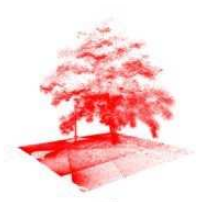
\includegraphics[width=\linewidth]{assets/2_5_a.png}
        \caption{{}}
        \label{fig:2.5a}
    \end{subfigure}
    \begin{subfigure}[H]{0.4\linewidth}
        \centering
        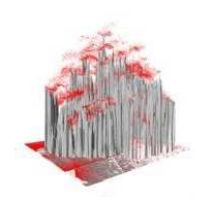
\includegraphics[width=\linewidth]{assets/2_5_b.png}
        \caption{{}}
        \label{fig:2.5b}
    \end{subfigure}
    \hfill
    \begin{subfigure}[H]{0.4\linewidth}
        \centering
        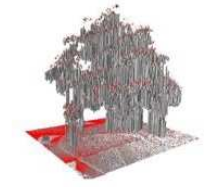
\includegraphics[width=\linewidth]{assets/2_5_c.png}
        \caption{{}}
        \label{fig:2.5c}
    \end{subfigure}
    \begin{subfigure}[H]{0.4\linewidth}
        \centering
        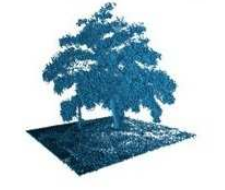
\includegraphics[width=\linewidth]{assets/2_5_d.png}
        \caption{{}}
        \label{fig:2.5d}
    \end{subfigure}
    \caption{Examples of a map represented in different structures. (a) Point cloud map. (b) Elevation map. (c) Multi-level surface map. (d) Occupancy grid map based on an octree. Image from [Hornung et al., 2013].}
    \label{fig:2.5}
\end{figure}
\subsubsection{Point cloud representation}
The point cloud is one of the simplest metric map representation of the environment (see Figure \ref{fig:2.5a}). The points gathered from a range sensor are transformed into a global coordinate frame. But, this representation is not adapted for dynamic environment and does not cope with sensor noise.
\subsubsection{Occupancy grid representation}
The occupancy grid map is a discretization of the environment in regularly sized 2D squares – called cells – or 3D cubic volumes – called voxels – (See Figure \ref{fig:2.5d}). The occupancy grid map is based on a hierarchical data structure – called Octree – which represents a 3D space that is recursively subdivided until attending a minimum voxel size – called resolution –(See Figure \ref{fig:2.6}). By increasing the resolution, the map becomes less coarser.
\begin{figure}[H]
    \centering
    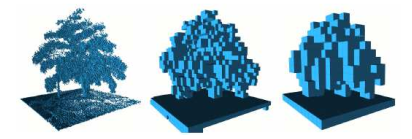
\includegraphics[width=\linewidth]{assets/2_6.png}
    \caption{Examples of an occupancy grid map with resolutions of $0.08m$, $0.64m$, and $1.28m$, respectively. Image from [Hornung et al., 2013].}
    \label{fig:2.6}
\end{figure}
The occupancy grid representation introduces several advantages [Hornung et al., 2013] such as:
\begin{itemize}
    \item Arbitrary environment representation without prior assumptions.
    \item Fast data access.
    \item Flexibility in extending and combining different maps with different resolutions.
    \item Updatability in adding new informations or sensor readings.
    \item Compact memory storage.
    \item Obstacle distinction for safe robot navigation.
\end{itemize}
Using the sensor measurements, the cells of the 2D (or the voxels of the 3D) occupancy grid map are labeled as unknown, free or occupied as shown in Figure \ref{fig:2.7}.
\begin{figure}[H]
    \centering
    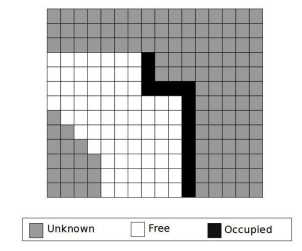
\includegraphics[width=\linewidth]{assets/2_7.png}
    \caption{2D occupancy grid example.}
    \label{fig:2.7}
\end{figure}
\paragraph{Occupancy grid matching}
We propose and implement a simple map matching process in order to evaluate and illustrate the global map during the mission. Suppose that we have two maps M 1 and M 2 (See Figure \ref{fig:2.8}) with the following assumptions:
\begin{itemize}
    \item Belonging to the same global frame.
    \item Having the same resolution.
\end{itemize}
\begin{figure}[H]
    \centering
    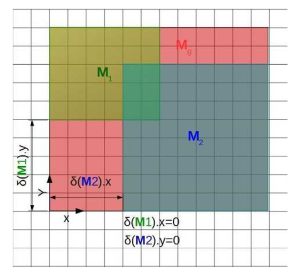
\includegraphics[width=\linewidth]{assets/2_8.png}
    \caption{Map matching of $\mathbf{M_1}$ and $\mathbf{M_2}$.}
    \label{fig:2.8}
\end{figure}
Each map is composed of:
\begin{itemize}
    \item \textit{Header}: It contains the sequence ID that is consecutively increasing, the stamp that defines the seconds and nanoseconds, and the frame this data is associated with.
    \item \textit{Meta data}: It contains the time load map, which is the time at which the map hasd been loaded, the map resolution ($\mathbf{M}_i.resolution$) that defines the metric size of the cells, the map width ($\mathbf{M}_i.width$) and height ($\mathbf{M}_i.heigth$) in number of cells, and the origin of the map ($\mathbf{M}_i.origin$).
    \item \textit{Data}: It contains the probability of occupancy of the cells in a row-major order.
\end{itemize}
Algorithm \ref{eq:2.1} describes the pipeline to match M 1 and M 2 where the steps can be summarized as follows:
\begin{itemize}
    \item Step 1 to 5: The meta data of the fused map are defined.
    \item Steps 6 to 7: Each cell in the fused map ($grid(\mathbf{M}_g)$) is initialized to $\mathbf{l}_u$ (cell labeled as $U N K N O W N $).
    \item Each unknown cell of the grid ($grid(\mathbf{M}_g)=\mathbf{l}_u$) is filled in using the value of either $grid(\mathbf{M}_1)$ or $grid(\mathbf{M}_2)$.
    \item Return the fused map $\mathbf{M}_g$
\end{itemize}
\begin{algorithm}
    \caption{Map matching.}
    \hspace*{\algorithmicindent} \textbf{Input:} Maps $\mathbf{M}_i$ with $i \in n_c$ \\
    \hspace*{\algorithmicindent} \textbf{Output:} Fused map $\mathbf{M}_g$
    \begin{algorithmic}[1]
        \STATE $\mathbf{M}_g.origin=argmin_{i \in n_c}(\mathbf{M}_i.origin);$
        \STATE $\delta(\mathbf{M}_i).x=\frac{(\mathbf{M}_g.origin.x-\mathbf{M}_i.origin.x)}{\mathbf{M}_i.resolution};$
        \STATE $\delta(\mathbf{M}_i).y=\frac{(\mathbf{M}_g.origin.y-\mathbf{M}_i.origin.y)}{\mathbf{M}_i.resolution};$
        \STATE $\mathbf{M}_g.width=argmax_{i \in n_c}(\mathbf{M}_i.width + \delta(\mathbf{M}_i).x);$
        \STATE $\mathbf{M}_g.height=argmax_{i \in n_c}(\mathbf{M}_i.height + \delta(\mathbf{M}_i).x);$
        \FOR {all grids in $\mathbf{M}_g$}
        \STATE $grid(\mathbf{M}_g)=\mathbf{l}_u$
        \FOR {$i=0;i<n_c;i++$}
        \FOR {$j=0;j<\mathbf{M}_i.width;j++$}
        \FOR {$k=0;k<\mathbf{M}_i.length;k++$}
        \IF {$grid(\mathbf{M}_i)\left[ j+k*\mathbf{M}_i.width \right]!=\mathbf{l}_u$}
        \STATE $grid(\mathbf{M}_g)\left[ (j-\delta(\mathbf{M}_i).x)+(k+\delta(\mathbf{M}_i).y)*\mathbf{M}_g.width \right]=grid\left[ j+k*\mathbf{M}_i.width \right]$
        \ENDIF
        \ENDFOR
        \ENDFOR
        \ENDFOR
        \ENDFOR
        \RETURN $\mathbf{M}_g.$
    \end{algorithmic}
\end{algorithm}
The proposed algorithm is a basic map matching approach used to merge two maps. It can be adapted to merge more than two maps at a time. This algorithm deals only with simple rectangular shape maps (This can be improved in our future work.).
\section{Monocular SLAM}
\subsection{Monocular sensor}
Monocular sensors are those where the only sensing device is a single camera. This sensor provides a set of images taken at discrete times k = [0..n] (See Eq.\ref{eq:2.4}).
\begin{equation} \label{eq:2.4}
    I_{0:n}=\{I_0,\dots,I_n\}
\end{equation}
Each image $I_k$ is a set of pixels – also called color components – that are stored in a $h \times w \times 3 $ matrix where the height $h$ and width $w$ of the image correspond to the matrix’s number of rows and columns, respectively (See Figure \ref{fig:2.9}). The element of $(u, v)$ index in the matrix represents the pixels’ RGB value.
\begin{figure}[H]
    \centering
    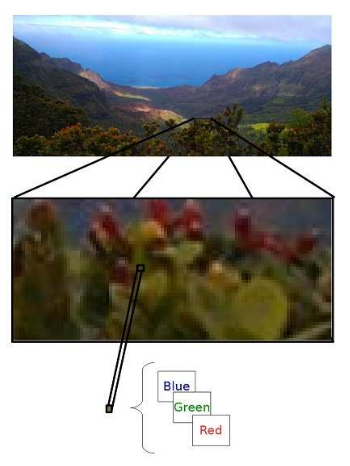
\includegraphics[scale=0.6]{assets/2_9.png}
    \caption{{Image\protect\footnotemark ~pixels representation}}
    \label{fig:2.9}
\end{figure}
\footnotetext{{This image was taken in Kauai Island, Hawaii.}}
\subsection{Visual SLAM}
Monocular sensors do not provide neither depth measurements (RGB-D camera example) nor two images of the same scene at the same time (stereo camera example) to compute these depth measurements. This leads to the inherent problem of scale ambiguity which consists in computing the scale factor. Despite the great progress in problems related to monocular SLAM, the main challenge is still the metric scale estimation. The scale\footnote{Source:\url{https://www.kudan.eu/kudan-news/scale-simultaneous-localisation-mapping/}} defines the relationship between sizes of the world and the created map. As a single camera cannot compute the scale factor, another sensor is added to be able to measure metrics from the environment. In the literature [Forster et al., 2015, Concha et al., 2016, Mur-Artal and Tardós, 2017b, Spaenlehauer et al., 2017], this additional sensor is mostly chosen to be an IMU due to its light weight, small size, and easiness to be mounted on an UAV.\\\\
An architecture for visual inertial SLAM system is proposed in Figure \ref{fig:2.10}. It uses a monocular camera and an IMU as sensors. Similarly to the PTAM approach [Klein and Murray, 2007], two threads are used: A tracker for a fast response to changes in the environment and a mapper to build a high quality map of the environment. The only difference is that the proposed approach uses odometry measurements instead of a motion model.
\begin{figure}[H]
    \centering
    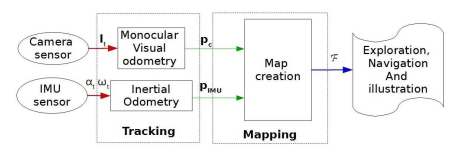
\includegraphics[scale=0.6]{assets/2_10.png}
    \caption{Visual inertial SLAM outline. $\mathbf{I}_t$ represent the images input sets from the camera. $\alpha_t$ and $\omega_t$ are, respectively, the acceleration and angular measurements from the IMU sensor. $\mathbf{p}_c$ and $\mathbf{p}_IMU$ are the estimated states from the camera and the IMU sensors, respectively. $\mathcal{F}$ is the generated 2D factor graph.}
\end{figure}
The monocular visual odometry is computed by detecting and tracking features of images coming from an extrinsic camera sensor. Additional inertial odometry is computed using the acceleration ($\alpha_t$) and the angular velocities ($\omega_t$) measurements from an intrinsic IMU sensor. Both are then fused in the mapper thread where a factor graph is created. An optimized pose estimation is then generated from this graph. For the map creation, a sparse nonlinear incremental optimization approach – called iSAM2 – [Kaess et al., 2012] is used. It allows to provide updated pose estimations when new measurements are available. \\\\
The proposed architecture allows not only to overcome the scale ambiguity but also to reduce the accumulated drift from the estimated trajectory.
\subsubsection{Problem formulation}
The proposed system is a graph-based SLAM problem that can be formulated in a factor graph. The graph is a factorization of a function $\mathbf{F}(\theta)$ described in Eq.\ref{eq:2.5}.
\begin{equation} \label{eq:2.5}
    \mathbf{F}(\theta)=\prod_i\mathbf{F}(\theta_i),
\end{equation}
with $\theta_i$ is a variable node $i$.\\\\
The purpose is to find the variable $\theta^*$ that maximizes the function $\mathbf{F}(\theta)$:
\begin{equation}\label{eq:2.6}
    \theta^*=argmax_\theta\mathbf{F}(\theta)
\end{equation}
The factor graph, presented in Figure \ref{fig:2.11} is composed of:
\begin{itemize}
    \item $\mathcal{P}_{0:n}=\{\mathbf{p}_0,\mathbf{p}_1,\dots,\mathbf{p}_n\}$: The set of unknown poses.
    \item $\mathcal{M}_{0:m}=\{\mathbf{m}_0,\mathbf{m}_1,\dots,\mathbf{m}_m\}$: The set of landmarks.
    \item $\mathcal{Z}_{i=cste,j=0:m}=\{\mathbf{z}_{i0},\mathbf{z}_{i1},\dots,\mathbf{z}_{im}\}$: The set of visual measurements.
    \item $\mathcal{B}_{0:n-1}=\{\mathbf{b}_0,\mathbf{b}_1,\dots,\mathbf{b}_{n-1}\}$: The set of odometry measurements. $\mathbf{b}_i$ is the odometry between the pose $\mathbf{p}_i$ and $\mathbf{p}_{i+1}$.
\end{itemize}
\begin{figure}[H]
    \centering
    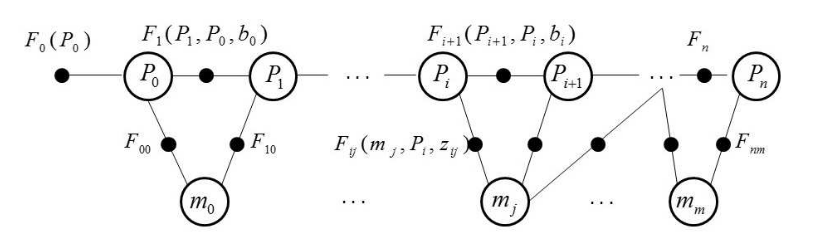
\includegraphics[scale=0.4]{assets/2_11.png}
    \caption{Factor graph for monocular SLAM. $\mathbf{F}_0(\mathbf{p}_0)$ and $\mathbf{m}_i$ are the variable nodes. $\mathbf{F}(0)$ is the prior density factor. $\mathbf{F}_{ij}(\mathbf{m}_j,\mathbf{p}_i,\mathbf{z}_{ij})$ is the odometry factor between the pose $\mathbf{p}_i$ and $\mathbf{F}_{ij}(\mathbf{m}_j,\mathbf{p}_i,\mathbf{z}_{ij})$ is the measurement likelihood model between the pose $\mathbf{p}_i$ and its landmark $\mathbf{m}_i$ .}
    \label{fig:2.11}
\end{figure}
This bipartite factor graph is composed of:
\begin{itemize}
    \item Variable node:
          \begin{itemize}
              \item Camera pose $\mathbf{p}_i$.
              \item Landmarks $\mathbf{m}_j$.
          \end{itemize}
    \item Factor nodes:
          \begin{itemize}
              \item Prior densities on the variable nodes $\mathbf{F}_0(\mathbf{p}_0)=p(\mathbf{p}_0)$.
              \item The motion models between two camera poses $\mathbf{F}_i(\mathbf{p}_{i+1},\mathbf{p}_i,\mathbf{b}_i)=p(\mathbf{p}_{i+1}|\mathbf{p}_i,\mathbf{b}_i)$ given the odometry measurement $\mathbf{b}_i$.
              \item The measurement likelihood models $\mathbf{F}_{ij}(\mathbf{m}_j,\mathbf{p}_i,\mathbf{z}_{ij})=p(\mathbf{m}_j|\mathbf{p}_j,\mathbf{z}_{ij})$ between the pose $\mathbf{p}_i$ and the landmark $\mathbf{m}_j$ given the visual measurement $\mathbf{z}_{ij}$.
          \end{itemize}
\end{itemize}
\subsubsection{Incremental Smoothing and Mapping 2 (iSAM2)}
To resolve the factor graph and estimate the poses, the iSAM2 approach [Kaess et al., 2012] is used. The estimation problem is based on three graphical models (See Figure \ref{fig:2.12}):
\begin{itemize}
    \item Explicit factor graph.
    \item Implicit chordal Bayes net.
    \item Bayes tree.
\end{itemize}
Therefore, the iSAM2 algorithm can incrementally obtain an estimate of unknown variables (such as UAV poses and landmarks) given a set of non linear factors (such as odometry) to finally construct the UAV’s map.
\begin{figure}[H]
    \centering
    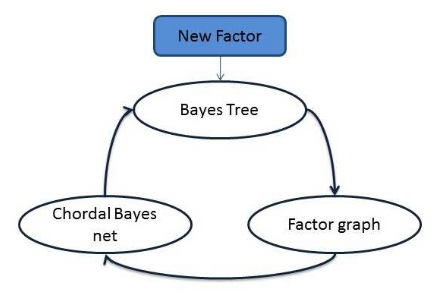
\includegraphics[scale=0.7]{assets/2_12.png}
    \caption{iSAM2 graphical models.}
    \label{fig:2.12}
\end{figure}
When a new factor is taken into account, the affected part of the Bayes Tree is isolated. From it, data are formulated as a factor graph and an associated Jacobian matrix. Then, the factor graph is transformed into a chordal Bayes net and a square root information matrix using a specific variable order elimination. The last one eliminated is called the root. Finally, based on the clique structure in the chordal Bayes net, a Bayes tree is formed with the square root information matrix. Based on these models, the incremental resolution and update of the iSAM2 are resumed in five important steps presented in Figure \ref{fig:2.13}.
\begin{figure}[H]
    \centering
    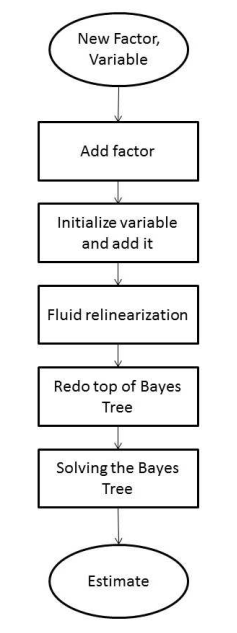
\includegraphics[scale=0.6]{assets/2_13.png}
    \caption{The iSAM2 steps.}
    \label{fig:2.13}
\end{figure}
Taking into account the available new factors, variables are initialized and added to the variable nodes. Thereafter, the process performs a fluid relinearization for marked variables in order to track the validity of the linearization point for each variable when needed. These marked variables are chosen according to a threshold between its current estimate and the linearization point. Then, the Bayes tree is partially updated starting from the cliques involved by the marked variables and the variables affected by new factors, up to the top of the tree. Using the obtained new Bayes tree, an update of the current estimate is performed.
\subsection{Results and discussions}
The SLAM algorithm was implement with the Georgia Tech Smoothing And Mapping toolbox\footnote{Source: \url{https://borg.cc.gatech.edu/index.html}} (GTSAM) using the factor graph implementation. The experimental code is written in MATLAB\footnote{Source: \url{https://fr.mathworks.com/}} and includes MEX functions\footnote{Source: \url{https://fr.mathworks.com/help/matlab/matlab_external/introducing-mex-files.html}} of the c++ library. Tests were performed on a 2.50GHz i5 Linux machine. To validate the SLAM algorithm, the measurements were simulated with raw data from the Kitti vision data-set Geiger et al., 2013. These data contain IMU measurements used for dead reckoning, and images used for the visual features. To compute the inter frame visual odometry, the libviso2 library\footnote{Source: \url{http://www.cvlibs.net/software/libviso/}} is used. Hence, given the set of non linear factors including IMU and visual odometry measurements, the iSAM2 estimates and optimizes poses and landmarks.\\\\
To see the improvement performed with the proposed approach, the estimated trajectory from iSAM2 is compared to those from IMU, libviso2 and GPS, in Figure \ref{fig:2.14}.
\begin{figure}[H]
    \centering
    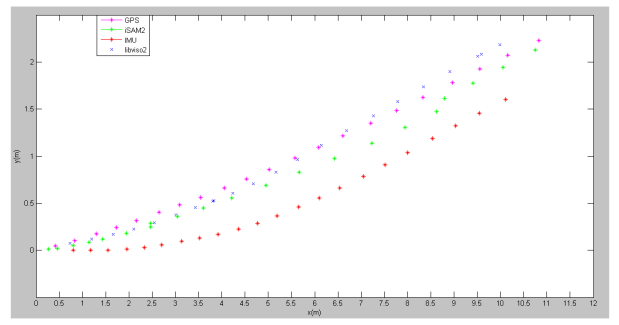
\includegraphics[scale=0.5]{assets/2_14.png}
    \caption{Trajectory results (2D projection) using IMU, libviso2, iSAM2 and GPS.}
    \label{fig:2.14}
\end{figure}
The GPS trajectory is obtained using Eq.\ref{eq:2.7}:
\begin{equation}\label{eq:2.7}
    \begin{split}
        x=R*\cos(latitude)*\cos(longtitude), \\
        y=R*\cos(latitude)*\sin(longtitude), \\
        z=R*\sin(latitude),
    \end{split}
\end{equation}
with $R$ the radius of the earth.\\\\
Results show that combining the IMU and the libviso2 trajectory using the iSAM2 helps to improve the poses estimation, and to reduce the IMU drift compared to the ground truth. Consequently, by obtaining a graph to exchange data instead of images, the data size is considerably reduced. Indeed, theoretically, sending images require about 1.843 Mbps (assuming that an image is encoded in 24 bits); whereas sending poses and landmarks needs about 0.323 Mbps (assuming that an IEEE standard encodes reals under 32 bits). Hence, thanks to the graph-based SLAM, we manage to reduce data size by about 5 times.
\section{RGB-D SLAM}
The RGB-D SLAM uses an RGB-D camera as a visual sensor to sense the environment.This sensor avoids the scale estimation problem thanks to the depth information.
\subsection{RGB-D sensor}
The RGB-D camera is composed of a digital camera for colored images $\mathbf{C}-t$ , and another device for the depth image $\mathbf{D}_t$ . The colored image $\mathbf{C}_t$ is a 3D matrix encoded in the RGB space where each color represents a dimension with a number of raws and columns corresponding to the image resolution (See section 1.3.1 on monocular sensor). The depth image $\mathbf{D}_t$ is a 2D matrix where $\mathbf{D}_t(u,v)$ is the depth of the pixel of column $u$ and row $v$. The depth measurements can be computed by different technologies (e.g. camera, infrared) where the RGB-D sensor can be classified as follows:
\begin{itemize}
    \item \textit{Active}: It is composed of a camera and a projector. The projector emits known patterns that are compared with the camera to get the correspondences. The depth is computed from these correspondences and the known transformation between the camera and the projector.
    \item \textit{Passive}: It represents stereo sensors composed of two RGB cameras. The depth is computed by knowing the transformation between them.
\end{itemize}
\textbf{RGB-D sensor Comparison}\\
Different types of RGB-D camera exist. One of the most famous is the kinect\footnote{Source: \url{https://msdn.microsoft.com/en-us/library/hh438998.aspx}} camera (See Figure \ref{fig:2.15a}). Other relatively new technologies are available such as DUO MLX\footnote{Source: \url{https://duo3d.com/product/duo-minilx-lv1}} (See Figure \ref{fig:2.15b}), ZED\footnote{Source: \url{https://www.stereolabs.com/zed/specs/}} stereo (See Figure \ref{fig:2.15c}), and Intel RealSense ZR300\footnote{Source: \url{https://software.intel.com/en-us/realsense/zr300}} (See Figure \ref{fig:2.15d}).
\begin{figure}[H]
    \centering
    \begin{subfigure}[H]{0.4\linewidth}
        \centering
        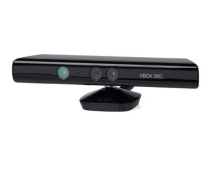
\includegraphics[width=\linewidth]{assets/2_15_a.png}
        \caption{{Kinect camera.}}
        \label{fig:2.15a}
    \end{subfigure}
    \begin{subfigure}[H]{0.4\linewidth}
        \centering
        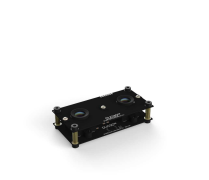
\includegraphics[width=\linewidth]{assets/2_15_b.png}
        \caption{{DUO MLX camera.}}
        \label{fig:2.15b}
    \end{subfigure}
    \begin{subfigure}[H]{0.4\linewidth}
        \centering
        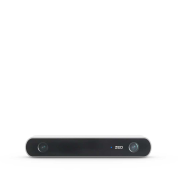
\includegraphics[width=\linewidth]{assets/2_15_c.png}
        \caption{{ZED camera}}
        \label{fig:2.15c}
    \end{subfigure}
    \begin{subfigure}[H]{0.4\linewidth}
        \centering
        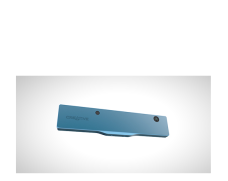
\includegraphics[width=\linewidth]{assets/2_15_d.png}
        \caption{{ZR300 camera.}}
        \label{fig:2.15d}
    \end{subfigure}
    \caption{Examples of RGB-D sensors.}
    \label{fig:2.15}
\end{figure}
A brief comparison is summarized in Table \ref{tab:2.1}. The ZED camera have the higher resolution and range compared to DUO and Kinect. However, this camera requires a powerful processor to work properly. DUO MLX is a lightweight camera with a good resolution, small dimensions but a small range and a relatively high price. The ZR300 has a small size and a good resolution but it is more expensive than the kinect. Despite its bigger dimension and weight, the kinect is the cheaper and the easiest to use. Taking into account the UAVs’ mission requirements and purpose, we make the choice to use the kinect. Yet, the SLAM algorithm is not restricted to a defined type of a RGB-D sensor.
% Please add the following required packages to your document preamble:
% \usepackage{graphicx}
\begin{table}[H]
    \caption{RGB-D sensors comparison}
    \label{tab:2.1}
    \resizebox{\textwidth}{!}{%
        \begin{tabular}{|l|l|l|l|l|}
            \hline
            \textbf{Characteristic}                 & \textbf{kinect xbox 360}       & \textbf{\begin{tabular}[c]{@{}l@{}}DUO MLX \\ (integrated IMU)\end{tabular}} & \textbf{ZED}                   & \textbf{ZR300}                 \\ \hline
            \textbf{\begin{tabular}[c]{@{}l@{}}Output\\  Resolution\end{tabular}} & \begin{tabular}[c]{@{}l@{}}640 x 480 x 24 \\ bpp 4:3 RGB\\ @30fps\\ 640 x 480 x 16\\ bpp 4:3 YUV\\ @15fps\end{tabular} & \begin{tabular}[c]{@{}l@{}}752 x 480 \\ @56fps\end{tabular}          & \begin{tabular}[c]{@{}l@{}}2x (1920 x 1080)\\  @30fps\end{tabular} & \begin{tabular}[c]{@{}l@{}}2 x VGA \\ @60fps\end{tabular} \\ \hline
            \textbf{\begin{tabular}[c]{@{}l@{}}Depth Range\\ (m)\end{tabular}} & 0.8 to 4.0                     & 0.23 to 2.5                             & 1 to 15                        & 0.4 to 2.8                     \\ \hline
            \textbf{\begin{tabular}[c]{@{}l@{}}Baseline\\ (mm)\end{tabular}} & 75                             & 30                                      & 120                            & 20                             \\ \hline
            \textbf{\begin{tabular}[c]{@{}l@{}}Dimensions \\ (mm)\end{tabular}} & 279 x 50,8 x 25                & 52 x 24 x 13                            & 175 x 30 x 33                  & \begin{tabular}[c]{@{}l@{}}9.5 x 101.56 \\ x 3.8\end{tabular} \\ \hline
            \textbf{\begin{tabular}[c]{@{}l@{}}Weight \\ (grams)\end{tabular}} & 750                            & 12.5                                    & 159                            & -                              \\ \hline
            \textbf{\begin{tabular}[c]{@{}l@{}}System \\ requirements\end{tabular}} & \begin{tabular}[c]{@{}l@{}}1.9 GHz CPU \\ 4GB RAM\end{tabular} & \begin{tabular}[c]{@{}l@{}}Modern \\ Processor\\ Intel i5/i7,\\ AMD or ARM\\ Minumum \\ 4GB RAM\end{tabular}          & \begin{tabular}[c]{@{}l@{}}Dual-core \\ 2.4GHz or\\ faster processor\\ Minumum \\ 4GB RAM\\ Nvidia GPU \\ with compute\\ capability \textgreater 3.0\end{tabular} & \begin{tabular}[c]{@{}l@{}}Intel Joule \\ compute \\ module with\\ Ubuntu 16.04\end{tabular} \\ \hline
            \textbf{price (\$)}                     & 33                             & 595                                     & 449                            & 129                            \\ \hline
        \end{tabular}%
    }
\end{table}
\subsection{Proposed approach}
The exploration task requires the UAV to implicitly maintain an accurate estimate of its pose in addition to a map of the observed environment. Figure \ref{fig:2.16} shows the outline of the localization and mapping processes. $\mathbf{C}_t$ and $\mathbf{D}_t$ represent, respectively, the colored and depth measurements gathered from the RGB-D sensor. $\mathbf{p}_i$ is the robot’s estimated pose, $\mathcal{P}_S$ represents the 3D point cloud computed by the SLAM system, and $\mathcal{O}$ and $\mathcal{L}$ contain the 3D and 2D grid map, respectively.
\begin{figure}[H]
    \centering
    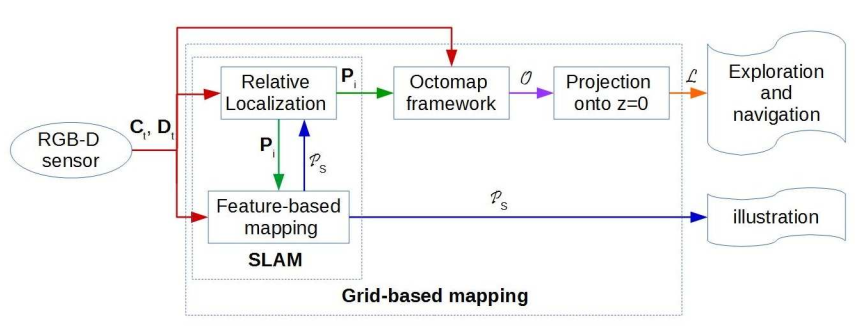
\includegraphics[scale=0.45]{assets/2_16.png}
    \caption{Localization and Mapping layers outline.}
    \label{fig:2.16}
\end{figure}
\subsubsection{SLAM module}
The SLAM module in Figure \ref{fig:2.16} provides an estimate of the robot’s 3D coordinates $\mathbf{p}_i$ w.r.t. the local reference frame $^WF_i$ (See Eq.\ref{eq:2.8}).
\begin{equation}\label{eq:2.8}
    \mathbf{p}_i=[x,y,z,q_x,q_y,q_z,q_w]^\top
\end{equation}
A sparse reconstruction of the environment is created using XYZ 3D point cloud. For pose estimation and map construction, among the existing RGB-D SLAM approaches, the ORB-SLAM2 vision-based framework [Mur-Artal and Tardós, 2017a] is used. This approach has shown promising results for pose estimation. The ORB-SLAM2 architecture is composed of threads and modules as represented in Figure \ref{fig:2.17}. It mainly contains:
\begin{itemize}
    \item Tracking thread for localization: To find and to match ORB feature, and to minimize the re-projection error.
    \item Local mapping thread for mapping: To optimize map using Bundle Adjustment.
    \item Loop closing thread in charge of detecting loops: To correct the accumulated drift using a pose graph optimization. This thread calls another thread in charge of performing full Bundle Adjustment (BA) to compute the optimal structure and the motion solution.
\end{itemize}
\begin{figure}[H]
    \centering
    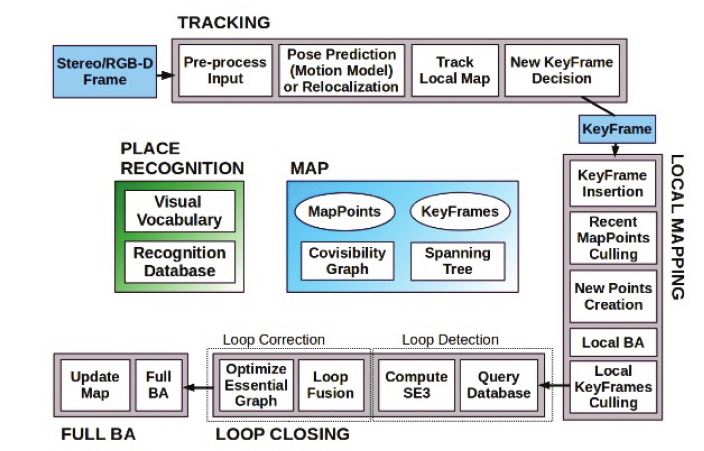
\includegraphics[scale=0.5]{assets/2_17.png}
    \caption{ORB-SLAM2 threads and modules. Image from [Mur-Artal and Tardos, 2017a].}
    \label{fig:2.17}
\end{figure}
These three main threads work in parallel. A place recognition module is used for relocalization and loop detection.
\subsubsection{Grid-based mapping module}
Using the estimated motion and the point cloud from the RGB-D sensor, a 3D occupancy grid is built during the grid-based mapping process (See Figure \ref{fig:2.16}). For that, the Octomap framework [Hornung et al., 2013] is used. It is a largely adopted 3D occupancy grid mapping framework. Furthermore, Octomap framework is able to perform grid mapping in challenging scenarios such as feature-less environment or fast camera motion [Endres et al., 2014]. Figure \ref{fig:2.18} shows an example of a desk environment representation using the Octomap framework.
\begin{figure}[H]
    \centering
    \begin{subfigure}[h]{0.4\linewidth}
        \centering
        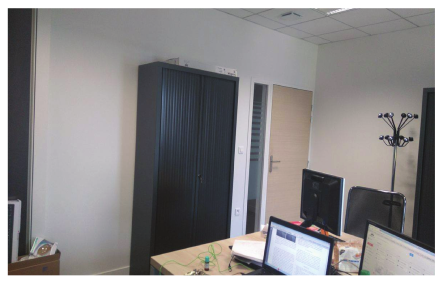
\includegraphics[width=\linewidth]{assets/2_18_a.png}
        \caption{{Real environment.}}
        \label{fig:2.18a}
    \end{subfigure}
    \hfill
    \begin{subfigure}[h]{0.4\linewidth}
        \centering
        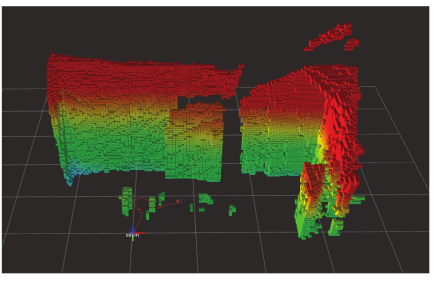
\includegraphics[width=\linewidth]{assets/2_18_b.png}
        \caption{{3D occupancy grid environment.}}
        \label{fig:2.18b}
    \end{subfigure}
    \caption{An example of environment representation using Octomap mapping framework (Resolution=0.05m).}
    \label{fig:2.18}
\end{figure}
The environment is approximated to a 3D voxels grid $\mathcal{O}$ where each voxel $\mathbf{o} \in \mathcal{O}$ is represented by its centroid (See Figure \ref{fig:2.19})
\begin{figure}[H]
    \centering
    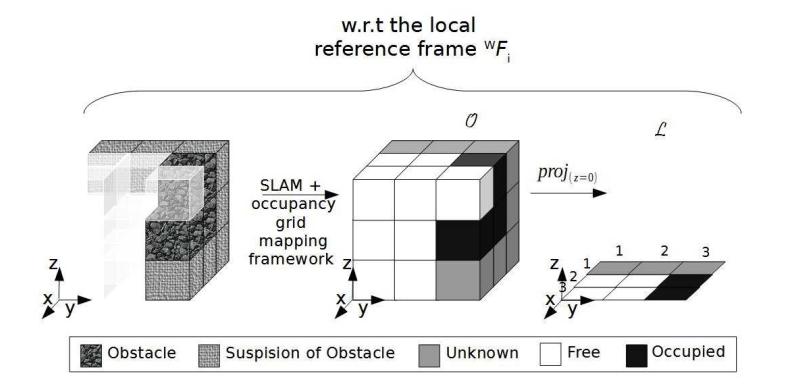
\includegraphics[scale=0.4]{assets/2_19.png}
    \caption{Map structure evolution during the SLAM process: From point cloud in the environment to 3D voxels $\mathcal{O}$ to 2D cells $\mathcal{L}$.}
    \label{fig:2.19}
\end{figure}
The visual sensor provides 3D point cloud to represent the environment. A 3D occupancy grid is then constructed by applying the SLAM approach and the occupancy grid mapping framework to the point cloud. Using the sensor measurements, voxels of the 3D occupancy grid map are labeled to unknown $\mathbf{o}_u$ , free $\mathbf{o}_u$ or occupied $\mathbf{o}_o$ . This 3D occupancy grid $\mathcal{O}$ is down-projected onto the plane $z = 0$ of the local frame $^WF_i$ to get a 2D cell grid $\mathcal{L}$ (See Equation \ref{eq:2.9}).
\begin{equation}\label{eq:2.9}
    \mathcal{L}=proj_{(z=0)}(\mathcal{O})
\end{equation}
The cells are occupied as soon as there is an occupied voxel in the $z$ cell range. And, they are free if all voxels in the $z$ cell range are so. Indeed, in a $z$ cell range, if there is occupied and unknown or free cells (See Equation \ref{eq:2.10}), the 2D projected cell will be occupied; now if there is unknown and free cells (See Equation \ref{eq:2.11}), the 2D projected cell will be unknown; and if there is only free cells (See Equation \ref{eq:2.12}), the 2D projected cell will be free.
\begin{eqnarray}
    \mathbf{l}_o(x,y)=\mathbf{o}_o(x,y,z)\wedge (\mathbf{o}_u(x,y,z)\vee \mathbf{o}_f(x,y,z)),\label{eq:2.10}\\
    \mathbf{l}_u(x,y)=\mathbf{o}_u(x,y,z)\wedge\mathbf{o}_f(x,y,z),\label{eq:2.11}\\
    \mathbf{l}_f(x,y)=\mathbf{o}_f(x,y,z),\label{eq:2.12}
\end{eqnarray}
Where $\wedge$ and $\vee$ represent AND (conjunction) and OR (disjunction) boolean operations, respectively.\\
Figure \ref{fig:2.20} shows the evolution of the map structure of an UAV that is executing a mission within a simulated environment. A Kinect camera is mounted on-board the UAV. These maps represent the sensed environment in the view frustum of the sensor at $t = 0s$, that is, at the beginning of the mission.
\begin{figure}[H]
    \centering
    \begin{subfigure}[t]{0.3\linewidth}
        \centering
        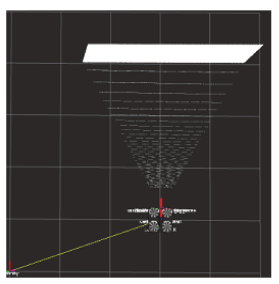
\includegraphics[width=\linewidth]{assets/2_20_a.png}
        \caption{{3D point cloud.}}
        \label{fig:2.20a}
    \end{subfigure}
    \begin{subfigure}[t]{0.3\linewidth}
        \centering
        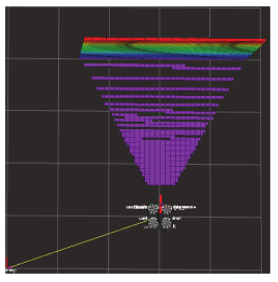
\includegraphics[width=\linewidth]{assets/2_20_b.png}
        \caption{{3D occupancy grid map.}}
        \label{fig:2.20b}
    \end{subfigure}
    \begin{subfigure}[t]{0.3\linewidth}
        \centering
        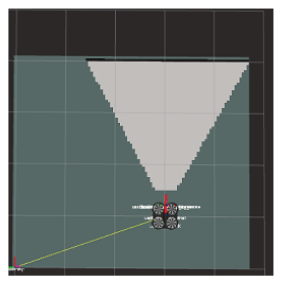
\includegraphics[width=\linewidth]{assets/2_20_c.png}
        \caption{{2D occupancy grid map.}}
        \label{fig:2.20c}
    \end{subfigure}
    \caption{Example of one UAV's map structure evolution.}
    \label{fig:2.20}
\end{figure}
\subsection{Result and discussions}
\subsubsection{Implementation details}
The simulations are performed using Robot Operating System\footnote{Source: \url{http://www.ros.org/}} (ROS) [Quigley et al., 2009] running on a 2.60GHz i7 Linux machine. For the quad-rotor simulaiton, the ARDrone model\footnote{Source: \url{http://wiki.ros.org/ardrone_autonomy}} equipped with an RGB-D camera in a forward-looking configuration, is used. A bounded unknown environment is generated using the $Gazebo$ simulator\footnote{Source: \url{http://gazebosim.org/}}. Figure \ref{fig:2.21} shows the implementation details related to the SLAM evaluation.
\begin{figure}[H]
    \centering
    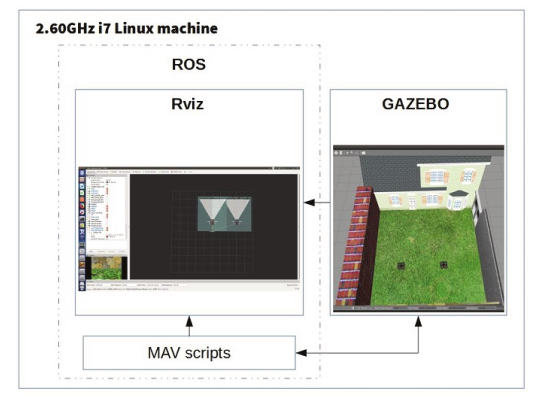
\includegraphics[scale=0.5]{assets/2_21.png}
    \caption{Implementation details of multiple UAVs on a single Linux machine}
    \label{fig:2.21}
\end{figure}
\subsubsection{Simulation results}
The ORB-SLAM2 approach [Mur-Artal and Tardós, 2017a] has been implemented and evaluated during an exploration mission\footnote{Source: \url{https://github.com/raulmur/ORB_SLAM2}} . Each robot runs its own ORB-SLAM2 within its local reference frame $^WF_i$ . Using the $Gazebo$ virtual environment and despite the need of structure and texture, the ORB-SLAM2 has been able to perform localization in a simulated area.
\paragraph{Parameters setting}
When using a relative localization, the motion is estimated by comparing the features in the current and previous frame. If the UAV’s speed is too high, the tracking of these features is lost. Thus, some parameters related to the UAV’s motion have been tuned. Table \ref{tab:2.2} resumes tests to set some of the required parameters (linear velocity $v_i$ and angular velocity $w_i$ ) to perform visual SLAM without tracking loss or – at least – a fast re-localization. For a tracking loss SLAM, the linear velocity $v_i$ is set to $[0.1, 0.2]m.s^{-1}$ and the angular velocity $w_i$ to $0.1rad.s^{-1}$
\begin{table}[H]
    \centering
    \caption{SLAM behavior while modifying linear and angular velocity. T.L: Tracking Loss; RL: Re-Localization.}
    \label{tab:2.2}
    \begin{tabular}{|l||*{3}{c|}}\hline
        \backslashbox{$v_i(m.s^{-1})$}{$w_i(rad.s^{-1})$}
            & \makebox[5em]{0.1} & \makebox[5em]{0.2} & \makebox[5em]{0.3}
        \\\hline
        0.1 & No T.L.            & No T.L.            & T.L., R.L.         \\\hline
        0.2 & No T.L.            & T.L., R.L.         & T.L.               \\\hline
        0.3 & T.L., R.L.         & T.L.               & T.L.               \\\hline
    \end{tabular}
\end{table}
\paragraph{SLAM performances using one UAV}
Figure \ref{fig:2.22} shows the SLAM system performances during one robot exploration. The drift as well as the trajectory errors are limited due to the loop-closure algorithm performed within ORB-SLAM2.
\paragraph{SLAM performances using two UAVs}
Results for exploration mission, using a fleet composed of two UAVs running each one the SLAM algorithm, are presented in Figure \ref{fig:2.23}. As expected, the exploration time using one UAV is greater than using two UAVs. An important drift occurs at the end of the $UAV_2$'s trajectory because it did not visit a known place and therefore it could not rectify its trajectory with a loop closure optimization.\\\\
Figure \ref{fig:2.22a} and Figure \ref{fig:2.23a} contain a 3D sparse point cloud along with robot trajectories computed by SLAM. The sparse representation of the environment is only used for illustration, not for exploration nor for navigation.
\begin{figure}[H]
    \centering
    \begin{subfigure}[t]{0.8\linewidth}
        \centering
        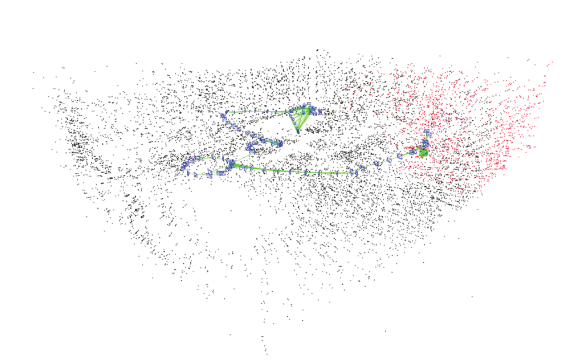
\includegraphics[width=\linewidth]{assets/2_22_a.png}
        \caption{{Sparce reconstruction of the environment. The blue markers represent the keyframes. The green lines represent the keyframe matching. The black and red points (present in the robot's current view frustum) represent the sparse recontruction of the environment.}}
        \label{fig:2.22a}
    \end{subfigure}
    \begin{subfigure}[t]{0.8\linewidth}
        \centering
        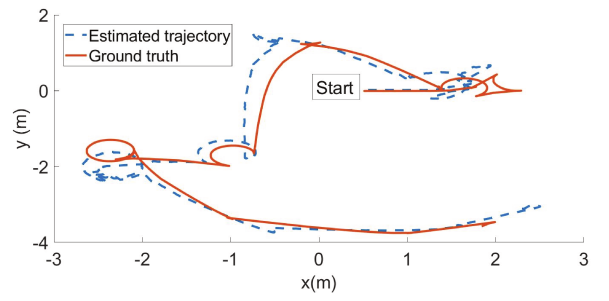
\includegraphics[width=\linewidth]{assets/2_22_b.png}
        \caption{{The estimated trajectory versus the Ground truth.}}
        \label{fig:2.22b}
    \end{subfigure}
    \begin{subfigure}[t]{0.8\linewidth}
        \centering
        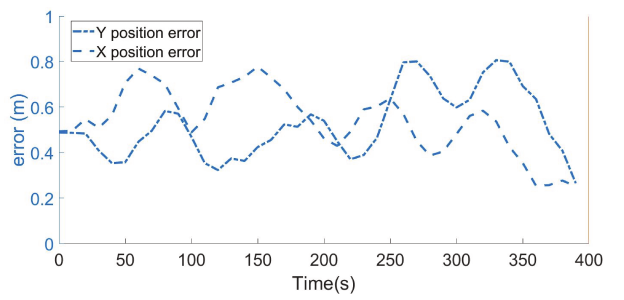
\includegraphics[width=\linewidth]{assets/2_22_c.png}
        \caption{{The estimated position errors during the mission.}}
        \label{fig:2.22c}
    \end{subfigure}
    \caption{One UAV exploration using SLAM algorithm. The kinect's maximum range is 4m, the UAV's linear velocity $v_i \in [0.1, 0.2]m.s^{-1}$ and angular velocity $w_i=0.1 rad.s^{-1}$. The RMSE(x)=0.2968 and RMSE(y)=0.2944}
    \label{fig:2.22}
\end{figure}
\begin{figure}[H]
    \centering
    \begin{subfigure}[t]{0.8\linewidth}
        \centering
        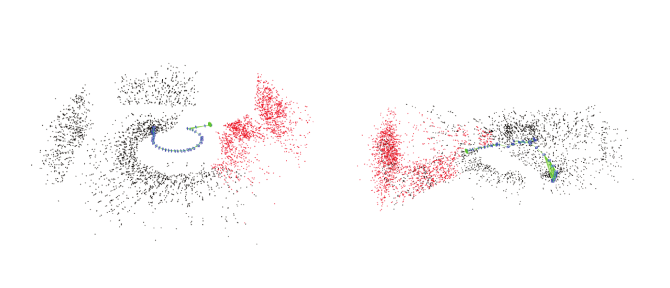
\includegraphics[width=\linewidth]{assets/2_23_a.png}
        \caption{{Sparce recontruction of the environment of UAV$_1$ (left) and UAV$_2$ (right). The blue markers represent the keyframes. The green lines represent the keyframe matching. The black and red points (present in the robot's current view frustum) represent the sparse reconstruction of the environment}}
        \label{fig:2.23a}
    \end{subfigure}
    \begin{subfigure}[t]{0.8\linewidth}
        \centering
        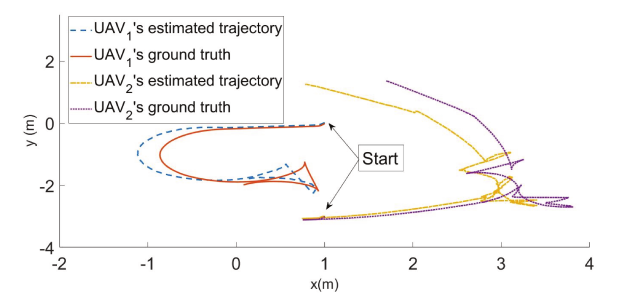
\includegraphics[width=\linewidth]{assets/2_23_b.png}
        \caption{{The estimated trajectory versus the Ground truth.}}
        \label{fig:2.23b}
    \end{subfigure}
    \begin{subfigure}[t]{0.8\linewidth}
        \centering
        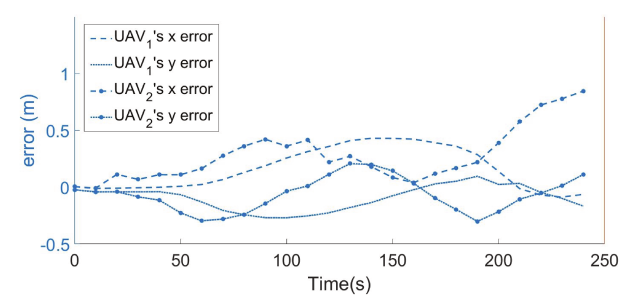
\includegraphics[width=\linewidth]{assets/2_23_c.png}
        \caption{{The estimated position errors during the mission.}}
        \label{fig:2.23c}
    \end{subfigure}
    \caption{Two UAVs cooperative exploration performing each one SLAM algorithm. The kinect's maximum range is 4m, the UAV's linear velocity $v_i \in [0.1, 0.2]m.s^{-1}$ and angular velocity $w_i=0.1 rad.s^{-1}$. For UAV$_1$, the RMSE(x)=0.2419 and RMSE(y)=0.1415; for UAV$_2$ the RMSE(x)=0.3649 and RMSE(y)=0.1614.}
    \label{fig:2.23}
\end{figure}
\section{Conclusion}
This chapter has addressed the problem of simultaneously determining the robot’s location and mapping the environment, while the robot moves. For that, a brief state of the art on the existing approaches have been presented. Then, we detailed two approaches for the SLAM problem.\\\\
A first approach was an inertial SLAM where a monocular camera was fused with an IMU. Results have shown that combining these two sensors improves the pose estimation and reduces the drift.\\\\
The second approach consists in using an RGB-D camera as the main sensor for SLAM. For that, the ORB-SLAM2 approach was implemented and evaluated using one and two UAVs in an exploration mission. Results has shown that the adopted approach allows to minimize the drift and consequently reduce the pose estimation error.\\\\
The RGB-D SLAM will be used in the next chapter as the relative localization algorithm for each UAV during the cooperative exploration missions.